\subsection{Terrain Generation Algorithms}

The main goal of this section is to provide an overview of the three algorithms that were implemented in our Web-based terrain generator for synthesis of realistic-looking terrains. Traditionally, procedural terrain generation focuses on the generation of a height for each point in a 2D space. In other words, it can be seen as function that maps \textit{x} and \textit{y} coordinates into \textit{z} coordinates: \[z=terrainGen(x, y)\]. Several techniques have built upon this height generation idea to create realistic-looking landscapes.

Two types of noise-based algorithms and one type of fractal-based algorithms are examined in this section, namely Perlin Noise (sometimes referred to as Perlin ``Classic'' Noise), Simplex Noise, and the Diamond Square algorithms. The first two were first described by Ken Perlin \cite{perlin:2002}, \cite{perlin:2001}, and the last one by Fournier, Fussell, and Carpenter \cite{fournier:1982}. These algorithms have since established themselves as a base from which various improvements have been suggested \cite{ong:2005, lechner:2006, pi:2006, li:2006, doran:2010} in the  procedural terrain generation field. An overview of each type is provided in the following subsections. 

\subsubsection{Perlin Noise}
The Perlin Noise is a procedurally generated visual effect developed by Ken Perlin \cite{perlin:2002}. It is a technique very useful in circumstances where computer memory is limited and users want to simulate elements from nature. The Perlin Noise works as follows:

\begin{enumerate}
\item It begins by creating a grid of vectors (gradients).
\item Each grid point has a gradient pointing away from it in a random direction (Figure~\ref{fig:randomGradients}).
\item For any given point (or pixel), interpolate the value from the surrounding N gradients. For a 2D space, the $N \eq 4$.
\item Finally, sum all values of the interpolations. Some example graphs generated by Perlin noise are show in Figure~\ref{fig:perlinEg}.
\end{enumerate}

Perlin noise can be created in 3D and higher dimensions. How do you do that? Well, you actually take slices along the z axis. Almost like a brain scan. You have a big 3D blob of noise and you just take thin slices and look at each one. Since each slice only changes a little, then it it looks like each slice animates all nicely.

\begin{figure}
	\center
	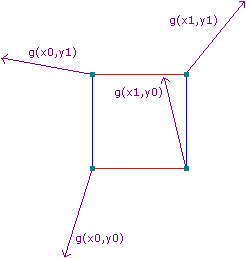
\includegraphics[scale=0.5]{images/gradients.png}
	\caption{Random Gradients}
	\label{fig:randomGradients}
\end{figure}
\begin{figure}
	\center
	\subfigure{
		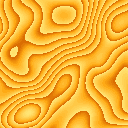
\includegraphics[scale=0.5]{images/woodgrain.png}
	}
	\subfigure{
		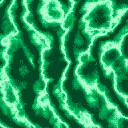
\includegraphics[scale=0.5]{images/marble.png}
	}
	\subfigure{
		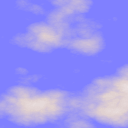
\includegraphics[scale=0.5]{images/clouds.png}
	}
	\caption{Perlin Noise Examples}
	\label{fig:perlinEg}
\end{figure}

The next algorithms to be described is the Simplex noise algorithm, which was developed by Ken Perlin \cite{perlin:2001} to overcome of the problems of the classic Perlin Noise.

\subsubsection{Simplex Noise}
Simplex noise is another noise generation algorithm developed by Perlin \cite{perlin:2001}. The goal of this algorithm is to make the noise generation simpler and faster, so that it could be implemented on hardware. In contrast to the Perlin's classic noise algorithm, the Simplex noise can scale to higher dimensions (4D, 5D and up) with much less computational cost. 

In 2D space, simplex noise differs from Perlin noise in the following ways:
\begin{enumerate}
	\item It uses a grid consisting of equilateral triangles instead of squares. As a result, there are only three adjacent grid points for each point in the space.
	\item Summation is used instead of interpolation. Simplex noise sums up the contributions from each corner (grid point) of the triangle, where ``the contribution is a multiplication of the extrapolation of the gradient ramp and a radially symmetric attenuation function'' \cite{Gustavson2005}. The calculation of summation is much less than interpolation, making simplex noise faster.
\end{enumerate}

Another approach for simulating realistic-looking landscapes is the diamond-square algorithm. Briefly, this algorithm is a midpoint displacement method that works by recursively calculating the missing values halfway among already known values and then randomly offsetting the new values inside a range, which has been determined by the current recursion depth. More details of this algorithm are described in the following subsection.

\subsubsection{Diamond-Square}
The Diamond-square algorithm is another method for generating height maps of artificial terrains. The difference between this algorithm and the above mentioned ones is that this algorithm uses fractals. 

This algorithm works on a 2D array of points; the number of points in each dimension should be $2^{n} + 1$, where $n$ is an integer. For example, $17 \times 17$, $1025 \times 1025$, etc). The algorithm starts by assigning seed values as heights to the four corners of a square, then it starts its iterative subdivision routine in two steps:

\begin{itemize}
	\item \textbf{The diamond step:} Average the heights of the four corners, add it to a random value and then assign the sum as the height of the square \textit{midpoint}, where two diagonals meet. The midpoints and corners form diamond shapes in the grid.
	\item \textbf{The square step:} Take each diamond of four points, average the heights of them and then add it to a random value in the same range of previous step to get the sum. Assign the sum to the midpoint of the diamond as the height. Once this done, it gives smaller squares again.
\end{itemize}

The iteration can repeat until all points in the grid have heights (Figure~\ref{fig:dsa}).

\begin{figure}
	\center
	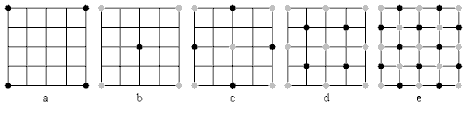
\includegraphics[scale=0.5]{images/dsa.png}
	\caption{Diamond-square Algorithm}
	\label{fig:dsa}
\end{figure}

\subsubsection{Combination of Algorithms}

Since all of the three algorithms described in this section accept \textit{x} and \textit{y} coordinates, and produce a height, we can combine these algorithms in different ways:

\begin{enumerate}
	\item Add up the height maps generated by several run of the same algorithm.
	\item Add up the height maps of different algorithms.
\end{enumerate}

By combining these algorithms, we are able to produce more interesting and complex terrains that just using individual algorithms; one at a time.

% subsection algorithms (end)